

% Stereographic and cylindrical map projections
% Author: Tomasz M. Trzeciak
% Source: LaTeX-Community.org 
%         <http://www.latex-community.org/viewtopic.php?f=4&t=2111>
\documentclass{standalone}
\usepackage{tikz}
\usetikzlibrary{calc,fadings,decorations.pathreplacing}
%% helper macros

\newcommand\pgfmathsinandcos[3]{%
  \pgfmathsetmacro#1{sin(#3)}%
  \pgfmathsetmacro#2{cos(#3)}%
}
\newcommand\LongitudePlane[3][current plane]{%
  \pgfmathsinandcos\sinEl\cosEl{#2} % elevation
  \pgfmathsinandcos\sint\cost{#3} % azimuth
  \tikzset{#1/.style={cm={\cost,\sint*\sinEl,0,\cosEl,(0,0)}}}
}
\newcommand\LatitudePlane[3][current plane]{%
  \pgfmathsinandcos\sinEl\cosEl{#2} % elevation
  \pgfmathsinandcos\sint\cost{#3} % latitude
  \pgfmathsetmacro\yshift{\cosEl*\sint}
  \tikzset{#1/.style={cm={\cost,0,0,\cost*\sinEl,(0,\yshift)}}} %
}
\newcommand\DrawLongitudeCircle[2][1]{
  \LongitudePlane{\angEl}{#2}
  \tikzset{current plane/.prefix style={scale=#1}}
   % angle of "visibility"
  \pgfmathsetmacro\angVis{atan(sin(#2)*cos(\angEl)/sin(\angEl))} %
  \draw[current plane] (\angVis:1) arc (\angVis:\angVis+180:1);
  \draw[current plane,dashed] (\angVis-180:1) arc (\angVis-180:\angVis:1);
}
\newcommand\DrawLatitudeCircle[2][1]{
  \LatitudePlane{\angEl}{#2}
  \tikzset{current plane/.prefix style={scale=#1}}
  \pgfmathsetmacro\sinVis{sin(#2)/cos(#2)*sin(\angEl)/cos(\angEl)}
  % angle of "visibility"
  \pgfmathsetmacro\angVis{asin(min(1,max(\sinVis,-1)))}
  \draw[current plane] (\angVis:1) arc (\angVis:-\angVis-180:1);
  \draw[current plane,dashed] (180-\angVis:1) arc (180-\angVis:\angVis:1);
}

%% document-wide tikz options and styles

\tikzset{%
  >=latex, % option for nice arrows
  inner sep=0pt,%
  outer sep=2pt,%
  mark coordinate/.style={inner sep=0pt,outer sep=0pt,minimum size=3pt,
    fill=black,circle}%
}
\begin{document}

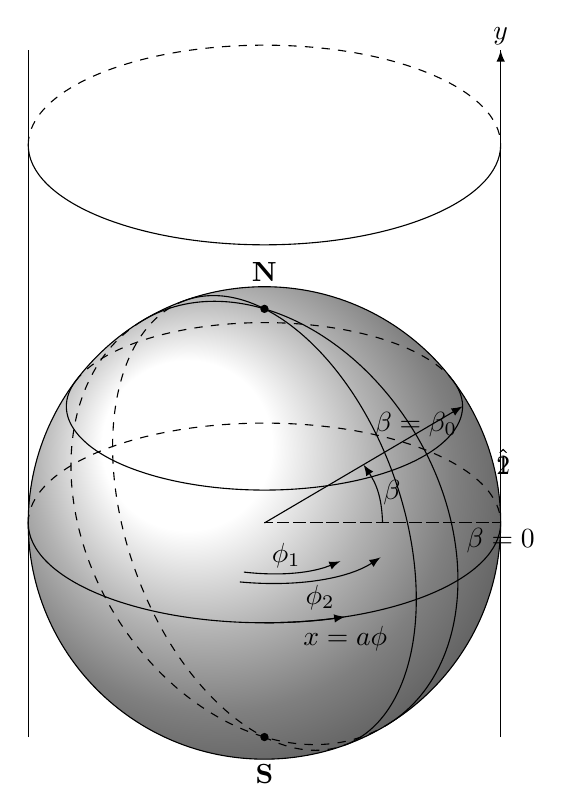
\begin{tikzpicture} % MERC

%% some definitions

\def\R{3} % sphere radius
\def\angEl{25} % elevation angle
\def\angAz{-100} % azimuth angle
\def\angPhiOne{-50} % longitude of point P
\def\angPhiTwo{-35} % longitude of point Q
\def\angBeta{33} % latitude of point P and Q

%% working planes

\pgfmathsetmacro\H{\R*cos(\angEl)} % distance to north pole
\LongitudePlane[xzplane]{\angEl}{\angAz}
\LongitudePlane[pzplane]{\angEl}{\angPhiOne}
\LongitudePlane[qzplane]{\angEl}{\angPhiTwo}
\LatitudePlane[equator]{\angEl}{0}

%% draw background sphere

\fill[ball color=white] (0,0) circle (\R); % 3D lighting effect
%\fill[white] (0,0) circle (\R); % just a white circle
\draw (0,0) circle (\R);

%% characteristic points

\coordinate (O) at (0,0);
\coordinate[mark coordinate] (N) at (0,\H);
\coordinate[mark coordinate] (S) at (0,-\H);
\path[xzplane] (\R,0) coordinate (XE);
\path[pzplane] (\angBeta:\R) coordinate (P);
\path[pzplane] (\R,0) coordinate (PE);
\path[qzplane] (\angBeta:\R) coordinate (Q);
\path[qzplane] (\R,0) coordinate (QE);

%% meridians and latitude circles

% \DrawLongitudeCircle[\R]{\angAz} % xzplane
% \DrawLongitudeCircle[\R]{\angAz+90} % yzplane
\DrawLongitudeCircle[\R]{\angPhiOne} % pzplane
\DrawLongitudeCircle[\R]{\angPhiTwo} % qzplane
\DrawLatitudeCircle[\R]{\angBeta}
\DrawLatitudeCircle[\R]{0} % equator

% shifted equator in node with nested call to tikz 
% (I didn't know it's possible)
\node at (0,1.6*\R) { \tikz{\DrawLatitudeCircle[\R]{0}} };

%% draw lines and put labels

\draw (-\R,-\H) -- (-\R,2*\R) (\R,-\H) -- (\R,2*\R);
\draw[->] (XE) -- +(0,2*\R) node[above] {$y$};
\node[above=8pt] at (N) {$\mathbf{N}$};
\node[below=8pt] at (S) {$\mathbf{S}$};
\draw[->] (O) -- (P);
\draw[dashed] (XE) -- (O) -- (PE);
\draw[dashed] (O) -- (QE);
\draw[pzplane,->,thin] (0:0.5*\R) to[bend right=15]
    node[midway,right] {$\beta$} (\angBeta:0.5*\R);
\path[pzplane] (0.5*\angBeta:\R) node[right] {$\hat{1}$};
\path[qzplane] (0.5*\angBeta:\R) node[right] {$\hat{2}$};
\draw[equator,->,thin] (\angAz:0.5*\R) to[bend right=30]
    node[pos=0.4,above] {$\phi_1$} (\angPhiOne:0.5*\R);
\draw[equator,->,thin] (\angAz:0.6*\R) to[bend right=35]
    node[midway,below] {$\phi_2$} (\angPhiTwo:0.6*\R);
\draw[equator,->] (-90:\R) arc (-90:-70:\R) node[below=0.3ex] {$x = a\phi$};
\path[xzplane] (0:\R) node[below] {$\beta=0$};
\path[xzplane] (\angBeta:\R) node[below left] {$\beta=\beta_0$};

\end{tikzpicture}
\end{document}
